%% -*- mode: latex; mode: flyspell -*-
\documentclass[12pt, letter]{article}

%% Class name and Assignment number
%%
\newcommand{\courseName}{Introduction~to~Deep~Learning~for~Computer~Vision}
\newcommand{\assignName}{Assignment~5:~PyTorch~Classifier~II}

%% Packages
\usepackage{amsmath,amsfonts,amssymb,amsthm,dsfont}
\usepackage{graphicx}
\usepackage[bookmarks=false]{hyperref}
\usepackage{color}
\usepackage{lipsum}

%% Paper format
\usepackage{geometry}
\geometry{
    letterpaper,
    %% total={216mm,279mm}, %< NSERC size
    margin=2.00cm,     %< default
    %% margin=1.87cm,       %< NSERC tightest
}

%% Headers and footers
\usepackage[explicit]{titlesec}
\newpagestyle{titlesec_assignment}{
  \sethead{\courseName}{}{\assignName}\setfoot{}{\thepage}{}
  \headrule
  %% \footrule
}

\graphicspath{ {./images/} }

\begin{document}

%% Set header and footer
\pagestyle{titlesec_assignment}

%% Title
\title{\courseName\\\assignName}
\author{Paul Molina-Plant}
\maketitle

\abstract{In this assignment I finished implementing the PyTorch classifer from
the previous assignment by implementing ReLU activation and adding the Test
mode. After finishing the implementation, I verified the accuracy and trained
the model with different parameters.}

\section{Implementing Solution}

To verify my implementation, I ran the model in test mode with the given
pretrained model and verified my accuracy against what was expected. My
test accuracy agreed with the expected result. \\

\begin{tabular}{lll}
  Configuration  & Test Accuracy & Loss  \\
  \hline
  Pretrained HoG & 59.93\%       & 1.295
\end{tabular}

\section{Testing configurations}
Next I trained the model with the following configurations. \\

\begin{tabular}{llll}
  Configuration  & Learning Rate & Units & Hidden Layers  \\
  \hline
  Model 1        & {1e-3}        & 64    & 3 \\
  Model 2        & {1e-4}        & 64    & 3 \\
  Model 3        & {1e-4}        & 128   & 3 \\
  Model 4        & {1e-4}        & 64    & 4 \\
  Model 5        & {1e-4}        & 128   & 4 \\
\end{tabular}

\pagebreak

  \subsection{Model 1}
  In model 1 I adjusted the learning rate to {1e-3}. \\

  From the plot, I determined this learning rate was too high, and chose to used
  {1e-4} for the remaining tests. In retrospect, the test accuracy for this
  model was slightly higher than model 2, so perhaps was not the correct choice. \\

  \begin{tabular}{lll}
    Configuration  & Test Accuracy & Loss  \\
    \hline
    Model 1        & 57.50\%        & 1.260
  \end{tabular}

  \begin{figure}[H]
    \centering
    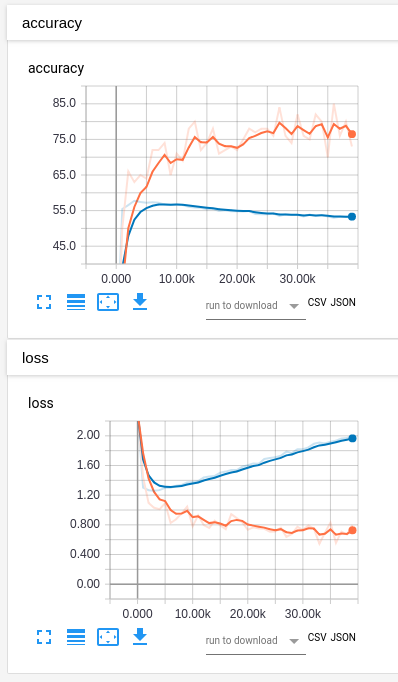
\includegraphics[width=0.8 \textwidth]{lr1e3}
    \caption{Model 1 Testing}
    \label{fig:eg}
  \end{figure}

  \subsection{Model 2}
  In model 1 I adjusted the learning rate to {1e-4}. \\

  \begin{tabular}{lll}
    Configuration  & Test Accuracy & Loss  \\
    \hline
    Model 2        & 56.41\%       & 1.300
  \end{tabular}

  \begin{figure}[H]
    \centering
    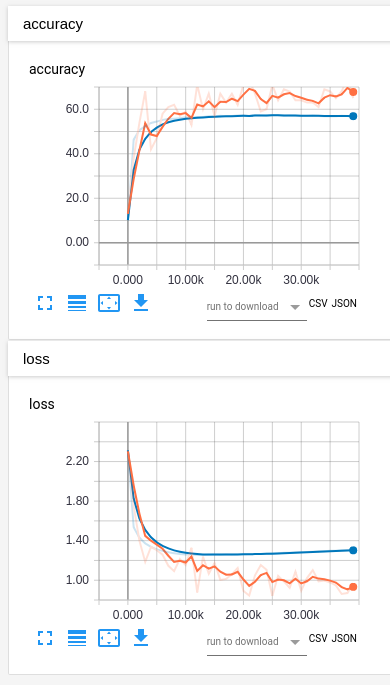
\includegraphics[width=0.8 \textwidth]{lr1e4}
    \caption{Model 2 Testing}
    \label{fig:eg}
  \end{figure}
  \subsection{Model 3}
  In model 1 I adjusted the learning rate to {1e-4} and the number of neurons
  per layer to 128. \\

  \begin{tabular}{lll}
    Configuration  & Test Accuracy & Loss  \\
    \hline
    Model 3        & 58.43\%       & 1.243
  \end{tabular}

  \begin{figure}[H]
    \centering
    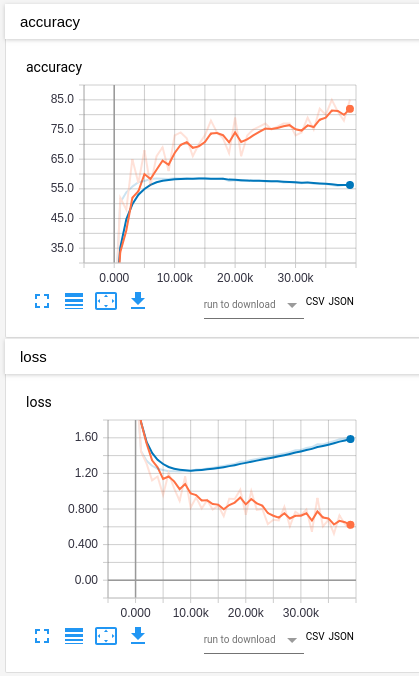
\includegraphics[width=0.8 \textwidth]{lr1e4unit128}
    \caption{Model 3 Testing}
    \label{fig:eg}
  \end{figure}

  \subsection{Model 4}
  In model 1 I adjusted the learning rate to {1e-4} and the number of hidden
  layers to 4. \\

  \begin{tabular}{lll}
    Configuration  & Test Accuracy & Loss  \\
    \hline
    Model 4        & 56.15\%        & 1.283
  \end{tabular}

  \begin{figure}[H]
    \centering
    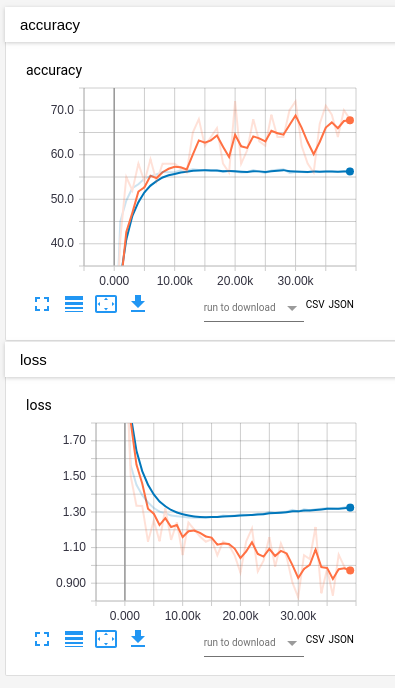
\includegraphics[width=0.8 \textwidth]{lr1e4hidden4}
    \caption{Model 4 Testing}
    \label{fig:eg}
  \end{figure}
  \subsection{Model 5}
  In model 1 I adjusted the learning rate to {1e-4}, the number of hidden layers
  to 4, and the number of neurons per layer to 128. \\

  \begin{tabular}{lll}
    Configuration  & Test Accuracy & Loss  \\
    \hline
    Model 5        & 58.03\%        & 1.269
  \end{tabular}

  \begin{figure}[H]
    \centering
    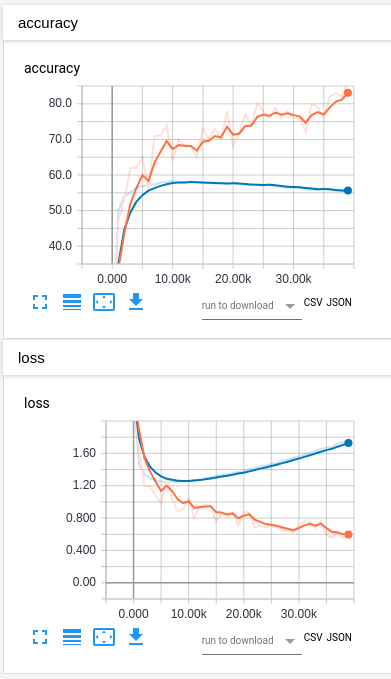
\includegraphics[width=0.8 \textwidth]{lr1e4hidden4unit128}
    \caption{Model 5 Testing}
    \label{fig:eg}
  \end{figure}

  \subsection{Conclusions}
  My model adjustments had at most a {2\%} difference
  on the final accuracy (model 3 to model 4). From these limited results, it
  appears that increasing the number of neurons correlates with increased
  accuracy. This is a reasonable conclusion because increasing the number of
  neurons enables the model to learn more detailed features, which would improve
  accuracy. Adding an additional hidden layer seemed to decrease the accuracy of
  the model, which I cannot explain.

\end{document}


%%% Local Variables:
%%% mode: latex
%%% TeX-master: t
%%% End:
